\documentclass[aps,prb,10pt,superscriptaddress,notitlepage]{revtex4-1}
\usepackage{grffile}
\usepackage{graphicx}
\usepackage[caption=false]{subfig}

\usepackage[colorlinks=true, linkcolor=blue, citecolor=red]{hyperref}

\begin{document}

\title{Convergence report for \emph{Plasmon dispersion in Graphite: A comparison
of current ab initio methods}}
\author{Sean M. Anderson}%\email{sma@cio.mx}
    \affiliation{Centro de Investigaciones en \'Optica, 
                Le\'on, Guanajuato, M\'exico}
\author{Bernardo S. Mendoza}%\email{bms@cio.mx}
    \affiliation{Centro de Investigaciones en \'Optica, 
                Le\'on, Guanajuato, M\'exico}
\author{Giorgia Fugallo}%\email{giorgia.fugallo@univ-nantes.fr}
    \affiliation{CNRS, UMR 6607, Laboratorie de Thermique et Energie de Nantes
    (LTeN) Polytech'Nantes, Universit\'e de Nantes, Rue Christian Pauc, F-44306
    Nantes Cedex 3, France}
\author{Francesco Sottile}%\email{francesco.sottile@polytechnique.fr}
    \affiliation{Laboratoire des Solides Irradi\'es, \'Ecole Polytechnique, 
    CNRS, CEA, Université Paris-Saclay, F-91128 Palaiseau, France }
    \affiliation{European Theoretical Spectroscopy Facility (ETSF)}
\date{\today}

\maketitle

In this report, we present a convergence study for the $q$-dependent EEL spectra
of graphite. The matter of convergence is an important one, since it is required
if we wish to accurately present these calculations. In particular, we are
interested in presenting the most accurate peak positions of the $\pi$ plasmon
(0--10\,eV energy range); namely Figs. 4, 5, and 7 of the main manuscript. We
will therefore restrict the energy range of the present convergence study
between 0--10\,eV. The range of frequencies where the $\pi + \sigma$ plasmon
occur, instead, is more delicate and while the RPA and TDDFT calculations well
converged with the parameters presented below, the full BSE CP is not in this
range. These results have been moved to the new Supplemental Material and serve
as qualitative benchmarks and trends.

Table \ref{tab:params} presents the relevant parameters for the calculations
featured in this work. The only exception, which is explicitely mentioned in the
main manuscript, is for the Bethe-Salpeter calculation including the coupling
terms in the excitonic Hamiltonian (BSE CP); for this method, we only use a
total of 20 bands instead of 80. However, as we demonstrate below, 20 total
bands is enough to accurately represent the 0--10\,eV energy range of the $\pi$
plasmon. Our convergence study for three select points along the
$\Gamma\rightarrow\mathrm{M}_{4}$ path as follows; Fig. \ref{fig:q0.00} is for
$q=0.00$ (at $\Gamma$), Fig. \ref{fig:q1.48} is for $q=1.48$\,\r{A}$^{-1}$ (at
M), and Fig. \ref{fig:q2.96} is for $q=2.96$\,\r{A}$^{-1}$ (at M in the fourth
Brillouin zone). The final parameters that were used throughout this work
(listed in Table \ref{tab:params}) are labeled on each figure. We have used a
Guassian broadening of 0.25\,eV for every result presented below, in order to
have a clear picture of the convergence behavior.

For $q=0.00$ (Fig. \ref{fig:q0.00}), we see that convergence is readily reached
for almost every parameter. Peak position differs by around $\sim0.1$\,eV for
the \textbf{k}-points (Fig. \ref{fig:q0.00_kpts}); the \textbf{k}-point grid
also determines what values of $q$ can be probed, so we must compromise between
the total number of \textbf{k}-points and the specific grid being used. For
$q=1.48$\,\r{A}$^{-1}$ (Fig. \ref{fig:q1.48}), the peak positions for the
various \textbf{k}-point grids remain almost unchanged (Fig.
\ref{fig:q1.48_kpts}), with very slight variation in peak intensity. For the
total number of bands (Fig. \ref{fig:q1.48_nband}), the selected 80 total bands
far exceeds the necessary number for convergence. We noted above that we used 20
total bands for the BSE CP calculation; at least for RPA, the intensity may be
slightly overestimated but the peak position remains virtually unchanged.

The situation is quite similar for $q=2.96$\,\r{A}$^{-1}$ (Fig.
\ref{fig:q2.96}); however, it becomes clear that the spectra are unconverged
with respect to the number of \textbf{k}-points (Fig. \ref{fig:q2.96_kpts}).
These curves indicate that convergence may require several thousand
\textbf{k}-points, which is well beyond our current computational capacity for
calculating the BSE CP spectra. That being said, it is very important to note
that Figs. 4, 5, and 7 of the main manuscript do not feature points beyond the
first Brillouin zone; thus, these results do not enter into that analysis.
Furthermore, the intensity is 1--2 orders of magnitude lower when compared to
the smaller values of $q$, so these results will not significantly impact the
heatmap plots presented in the main manuscript and supplemental material. The
same is true for the experimental counterpart: the intensity of the electron
energy loss signal decay as $\frac{1}{q^2}$ with increasing \textbf{q}.

In conclusion, we consider that the calculations presented in this work are more
than adequately converged. We would like to point out that, even though the
convergence study has been carried out in RPA (and ALDA), the very same holds
true for BSE. BSE calculations, in fact, converge at the same pace of RPA,
sometimes even faster (e.g. with respect to the number of bands).

%%%%%%%%%%%%%%%%%%%%%%%%%%%%%%%%%%%%%%%%%%%%%%%%%%%%%%%%%%%%%%%%%%%%%%%%%%%%%%%%
%%%%%%%%%%%%%%%%%%%%%%%%%%%%%%%%%%%%%%%%%%%%%%%%%%%%%%%%%%%%%%%%%%%%%%%%%%%%%%%%

\begin{table}
\caption{Calculation parameters used throughout this work.}
\label{tab:params}
\begin{ruledtabular}
\begin{tabular}{ l c c }
Parameter               & Variable  & Value \\
\hline
Cutoff energy (Ha)      & ecut      & 20 \\
\textbf{k}-points       & kpts      & 288 (12$\times$12$\times$02),
                                      392 (14$\times$14$\times$02) \\
Total number of bands   & nbands    & 80 (20) \\
G-vector shells         & matsh     & 12 \\
Wavefunction shells     & wfnsh     & 20
\end{tabular}
\end{ruledtabular}
\end{table}

%%%%%%%%%%%%%%%%%%%%%%%%%%%%%%%%%%%%%%%%%%%%%%%%%%%%%%%%%%%%%%%%%%%%%%%%%%%%%%%%
%%%%%%%%%%%%%%%%%%%%%%%%%%%%%%%%%%%%%%%%%%%%%%%%%%%%%%%%%%%%%%%%%%%%%%%%%%%%%%%%

\begin{figure}%
\centering
\subfloat[Cutoff energy\label{fig:q0.00_ecut}]
{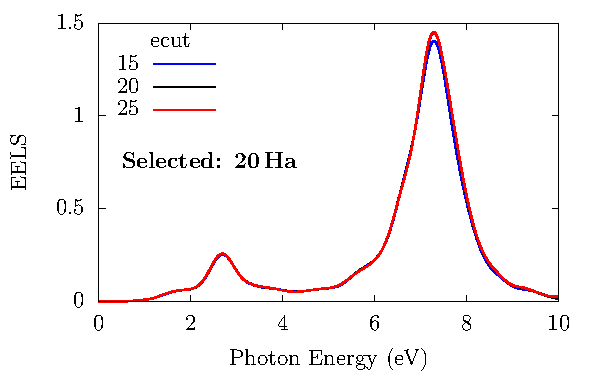
\includegraphics[width=0.45\linewidth]{figures/conv-q0.00-00ecut}}%
~
\subfloat[\textbf{k}-points\label{fig:q0.00_kpts}]
{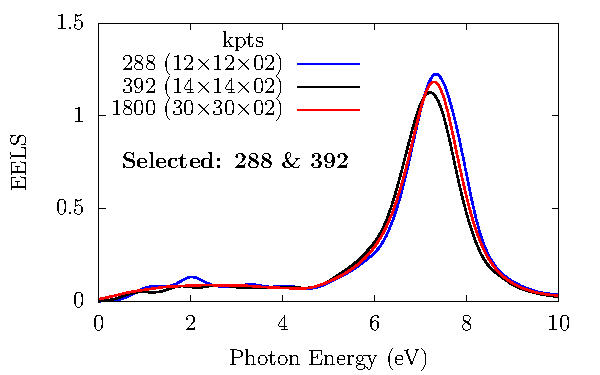
\includegraphics[width=0.45\linewidth]{figures/conv-q0.00-01kpts}}
\\
\subfloat[Total number of bands\label{fig:q0.00_nband}]
{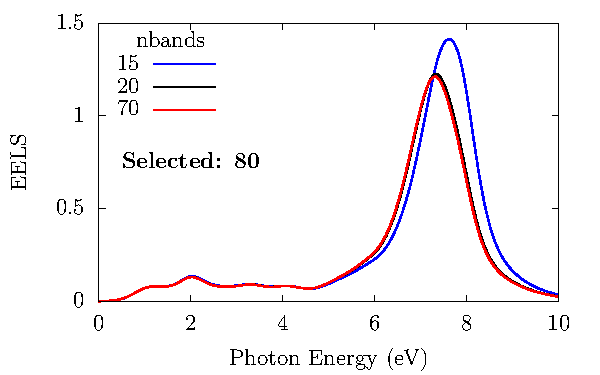
\includegraphics[width=0.45\linewidth]{figures/conv-q0.00-02nband}}%
~
\subfloat[G-vector shells\label{fig:q0.00_matsh}]
{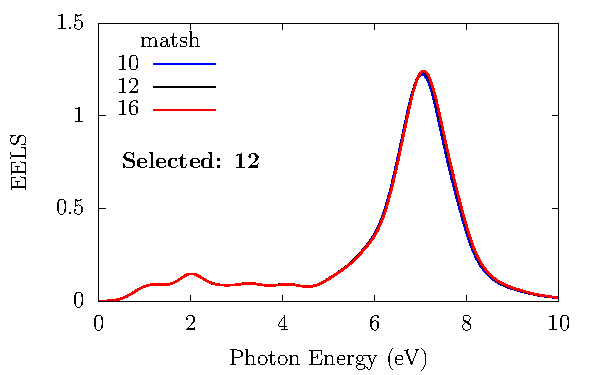
\includegraphics[width=0.45\linewidth]{figures/conv-q0.00-03matsh}}
\\
\subfloat[Wavefunction shells\label{fig:q0.00_wfnsh}]
{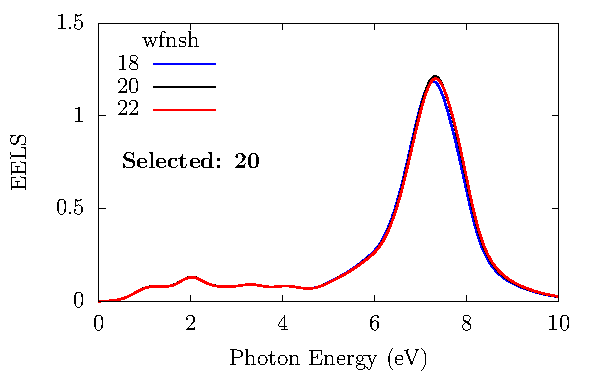
\includegraphics[width=0.45\linewidth]{figures/conv-q0.00-04wfnsh}}
\caption{Convergence for $q=0.00$ $\big(0\,\,\,0\,\,\,0\big)$.}%
\label{fig:q0.00}%
\end{figure}

%%%%%%%%%%%%%%%%%%%%%%%%%%%%%%%%%%%%%%%%%%%%%%%%%%%%%%%%%%%%%%%%%%%%%%%%%%%%%%%%
%%%%%%%%%%%%%%%%%%%%%%%%%%%%%%%%%%%%%%%%%%%%%%%%%%%%%%%%%%%%%%%%%%%%%%%%%%%%%%%%

\begin{figure}%
\centering
\subfloat[Cutoff energy\label{fig:q1.48_ecut}]
{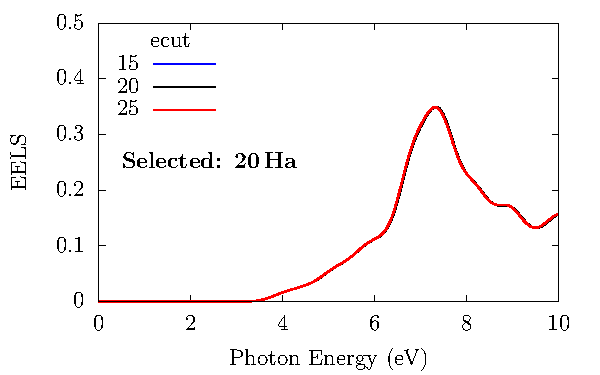
\includegraphics[width=0.45\linewidth]{figures/conv-q1.48-00ecut}}%
~
\subfloat[\textbf{k}-points\label{fig:q1.48_kpts}]
{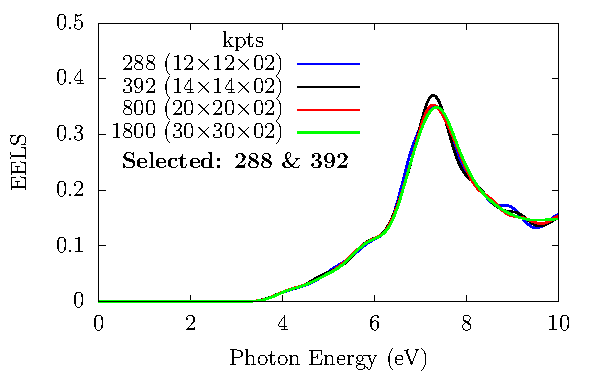
\includegraphics[width=0.45\linewidth]{figures/conv-q1.48-01kpts}}
\\
\subfloat[Total number of bands\label{fig:q1.48_nband}]
{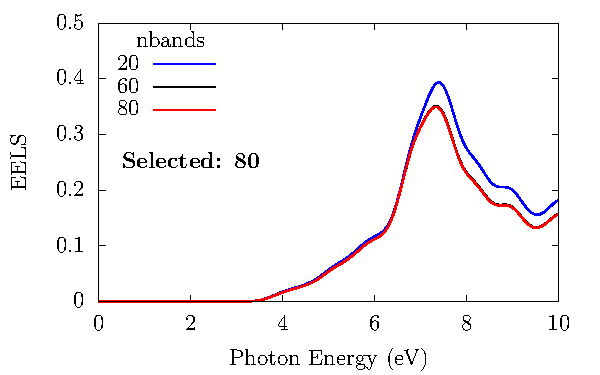
\includegraphics[width=0.45\linewidth]{figures/conv-q1.48-02nband}}%
~
\subfloat[G-vector shells\label{fig:q1.48_matsh}]
{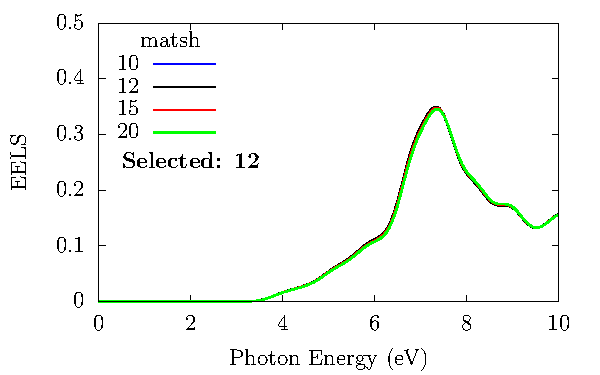
\includegraphics[width=0.45\linewidth]{figures/conv-q1.48-03matsh}}
\\
\subfloat[Wavefunction shells\label{fig:q1.48_wfnsh}]
{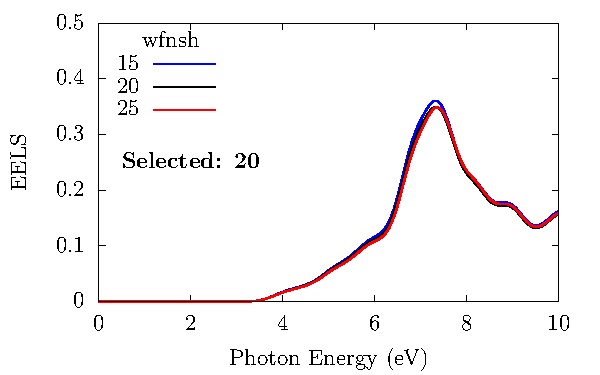
\includegraphics[width=0.45\linewidth]{figures/conv-q1.48-04wfnsh}}
\caption{Convergence for $q=1.48$\,\r{A}$^{-1}$
$\big(\frac{1}{2}\,\,\,0\,\,\,0\big)$.}%
\label{fig:q1.48}%
\end{figure}

%%%%%%%%%%%%%%%%%%%%%%%%%%%%%%%%%%%%%%%%%%%%%%%%%%%%%%%%%%%%%%%%%%%%%%%%%%%%%%%%
%%%%%%%%%%%%%%%%%%%%%%%%%%%%%%%%%%%%%%%%%%%%%%%%%%%%%%%%%%%%%%%%%%%%%%%%%%%%%%%%

\begin{figure}%
\centering
\subfloat[Cutoff energy\label{fig:q2.96_ecut}]
{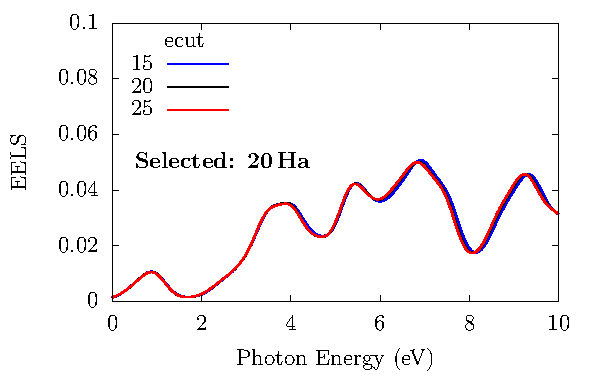
\includegraphics[width=0.45\linewidth]{figures/conv-q2.96-00ecut}}%
~
\subfloat[\textbf{k}-points\label{fig:q2.96_kpts}]
{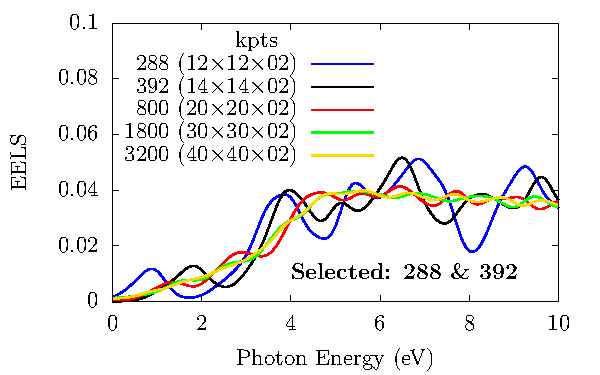
\includegraphics[width=0.45\linewidth]{figures/conv-q2.96-01kpts}}
\\
\subfloat[Total number of bands\label{fig:q2.96_nband}]
{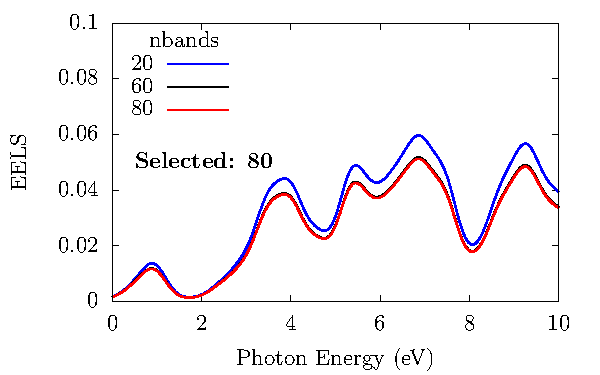
\includegraphics[width=0.45\linewidth]{figures/conv-q2.96-02nband}}%
~
\subfloat[G-vector shells\label{fig:q2.96_matsh}]
{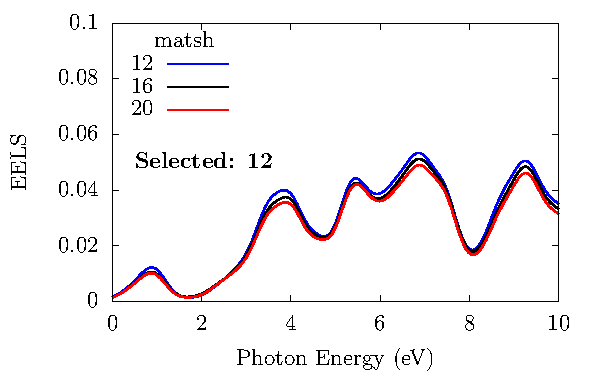
\includegraphics[width=0.45\linewidth]{figures/conv-q2.96-03matsh}}
\\
\subfloat[Wavefunction shells\label{fig:q2.96_wfnsh}]
{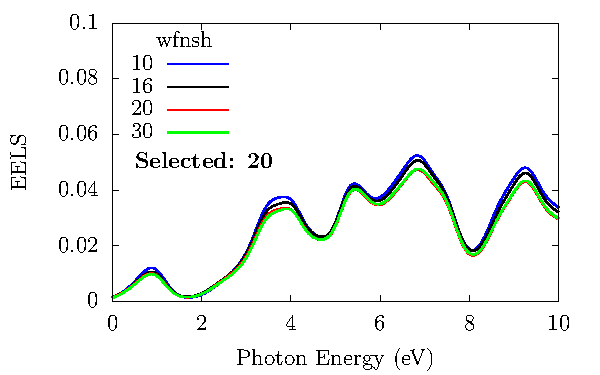
\includegraphics[width=0.45\linewidth]{figures/conv-q2.96-04wfnsh}}
\caption{Convergence for $q=2.96$\,\r{A}$^{-1}$ $\big(1\,\,\,0\,\,\,0\big)$.}%
\label{fig:q2.96}%
\end{figure}

\end{document}
